\documentclass{beamer}

\usepackage[utf8]{inputenc}
\usetheme{Warsaw}

\title{Embedded Systems - Bachelor Project}
\author{Moritz Herzog, Philipp Lersch}
\date{\today}

\usepackage{tikz}
\usetikzlibrary{shapes.geometric, arrows, chains, calc}

\tikzset{
    green/.style  = {draw, rectangle, minimum width=2cm, minimum height=1cm, text centered, text width=1.2cm, font=\footnotesize, draw=black, fill=green!30},
    blue/.style   = {draw, rectangle, minimum width=8cm+3\pgflinewidth, minimum height=1cm, text centered, text width=5.0cm, font=\footnotesize, draw=black, fill=blue!30},
    yellow/.style = {draw, rectangle, minimum width=8cm+3\pgflinewidth, minimum height=1cm, text centered, text width=5.0cm, font=\footnotesize, draw=black, fill=yellow!30},
}

\addtobeamertemplate{navigation symbols}{}{%
    \usebeamerfont{footline}%
    \usebeamercolor[fg]{footline}%
    \hspace{1em}%
    \insertframenumber/\inserttotalframenumber
}

\AtBeginSection[]
{
  \begin{frame}
    \frametitle{Table of Contents}
    \tableofcontents[currentsection]
  \end{frame}
}

\begin{document}
\maketitle


\section{OpenCL}
\begin{frame}
    \frametitle{OpenCL Structure}
    \begin{columns}
        \column{.6\textwidth}
        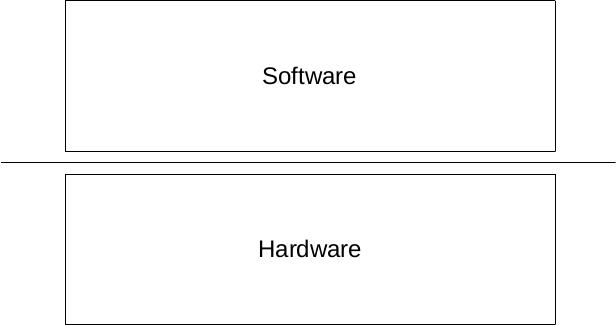
\includegraphics[width=\textwidth]{res/HardwareSoftwareLayer.jpg}
        \column{.4\textwidth}
        \begin{itemize}
            \item OpenCL draws clear line between hardware and software
            
        \end{itemize}
    \end{columns}
\end{frame}
\subsection{Hardware Model}
\begin{frame}
    \frametitle{Hardware Model}
    \begin{itemize}
     \item Diffrent Models for CPU and GPU
    \end{itemize}
\end{frame}
\begin{frame}
    \frametitle{Hardware Model - Memory}
    \begin{itemize}
     \item Some Memeory Stuff
    \end{itemize}
\end{frame}
\begin{frame}
    \frametitle{Hardware Model - CPU}
    \begin{itemize}
     \item Some CPU Stuff
    \end{itemize}
\end{frame}
\begin{frame}
    \frametitle{Hardware Model - GPU}
    \begin{itemize}
     \item Some GPU Stuff
    \end{itemize}
\end{frame}
\subsection{Software Model}
\begin{frame}
    \frametitle{Software Model}
\end{frame}

\section{Kernels}
\begin{frame} %%Eine Folie
  \frametitle{List of Kernels} %%Folientitel
  Already there:
  \begin{itemize}
   \item Battery
   \item Speed
   \item Acceleration
   \begin{itemize}
    \item X-Achsis
    \item Y-Achsis
    \item Tangential
   \end{itemize}
   \item Tempreture
  \end{itemize}

  %\begin{Definition} %%Definition
  %  Eine Definition
  %\end{Definition}
\end{frame}
\begin{frame}
    \frametitle{List of Kernels}
    Added Kernels:
    \begin{itemize}
     \item Tractioncontrol
     \item Accident Detection
     \item Anti-Lock Braking System
    \end{itemize}
\end{frame}
\subsection{Tractioncontrol}
\begin{frame}
    \frametitle{Tractioncontrol}
    The assumption is that the drive is on the rear axle.
    Alorthmical Description:
    \begin{itemize}
     \item Check if rear right wheel is spinning much faster (threshold is around 40\%) than rear left.\\
     $\Rightarrow$ Rear right wheel has no Traction.\\
     $\Rightarrow$ Stop Engine and lock the differential and inform diver.
     \pause
     \item Check if rear left wheel is spinning much faster than rear left.\\
     $\Rightarrow$ Rear left wheel has no Traction. $\Rightarrow$ Same reaction as left wheel.
     \pause
     \item Check if both wheels are spinning much faster than the front axel.\\
     $\Rightarrow$ Slow down the Engine.
    \end{itemize}
\end{frame}
\subsection{Accident Detection}
\begin{frame}
 %TODO To be filled
\end{frame}
\subsection{Anti-Lock Braking System}
\begin{frame}
 %TODO To be filled
\end{frame}
\subsection{Range}
\begin{frame}
 %TODO To be filled
\end{frame}
\end{document}
